\chapter{\ifproject%
\ifenglish Project Structure and Methodology\else โครงสร้างและขั้นตอนการทำงาน\fi
\else%
\ifenglish Project Structure\else โครงสร้างของโครงงาน\fi
\fi
}

ในบทนี้จะกล่าวถึงหลักการ และการออกแบบระบบ

\makeatletter

% \renewcommand\section{\@startsection {section}{1}{\z@}%
%                                    {13.5ex \@plus -1ex \@minus -.2ex}%
%                                    {2.3ex \@plus.2ex}%
%                                    {\normalfont\large\bfseries}}

\makeatother
%\vspace{2ex}
% \titleformat{\section}{\normalfont\bfseries}{\thesection}{1em}{}
% \titlespacing*{\section}{0pt}{10ex}{0pt}

\section{โครงสร้างของระบบ}

ภาพรวมโครงสร้างของระบบ จะเป็นดังรูปนี้

\begin{figure}[H]
  \begin{center}
  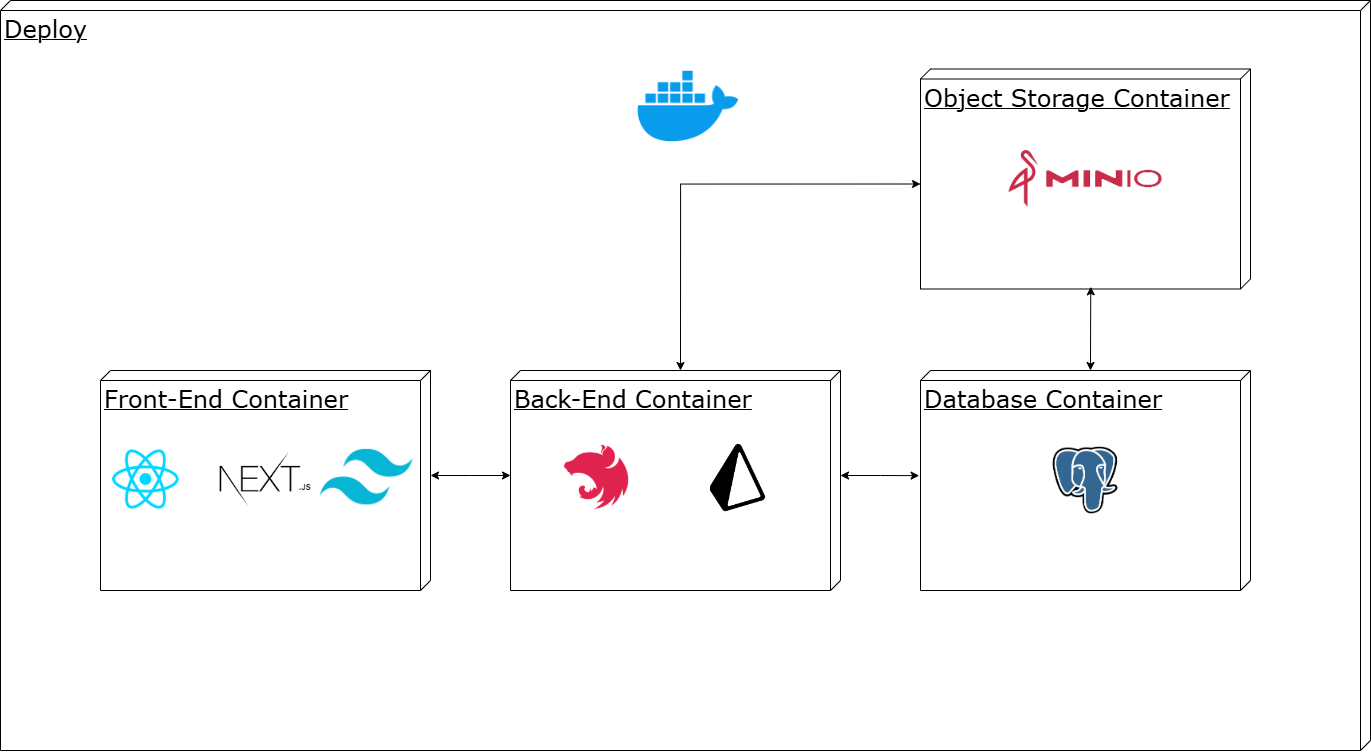
\includegraphics[width=1\textwidth]{Untitled Diagram.drawio (3).png}
  \end{center}
  \caption[โครงสร้างของระบบ]{โครงสร้างของระบบ}
\end{figure}
\subsection{Front-end}
\begin{itemize}
\item เลือกใช้ Next.js และ React เพราะมีความสำเร็จรูปในตัวเอง มีเครื่องมือที่มีให้ใช้พร้อม และยังเป็นที่ใช้แพร่หลาย ทำให้สามารถค้นหาข้อมูลเกี่ยวกับ Framework ได้ง่าย
\item เลือกใช้ Tailwind CSS เพราะเป็น component สำเร็จรูปที่สามารถ custom ได้ง่ายและเป็นที่นิยม
\end{itemize}
\subsection{Back-end}
\begin{itemize}
\item เลือกใช้ Nest JS เพราะมีความสำเร็จรูปในตัวเอง มีเครื่องมือที่พร้อมใช้งานได้เลยโดยไม่ต้องสร้างเพิ่ม 
\item เลือกใช้ MinIO เพราะเหมาะสำหรับกรณีที่ต้องการตัวเลือกการจัดเก็บข้อมูลที่มีความเร็วสูงและมีต้นทุนต่ำ สามารถใช้งานในระบบคลาวด์หรือเซิร์ฟเวอร์ขององค์กรได้ โดยไม่ต้องพึ่งพาผู้ให้บริการคลาวด์
\end{itemize}
\newpage
\subsection{Database และ Object Storage}
\begin{itemize}
\item เลือกใช้ PostgreSQL เพราะเหมาะกับข้อมูลขนาดใหญ่ ทำงานได้ดีในการอ่าน หรือ เขียน และ การวิเคราะห์ข้อมูลอย่างละเอียด 
\item เลือกใช้ Prisma เพราะมี Learning Curve ที่สูง ใช้งานง่าย และมีประสิทธิภาพดีเท่ากับตัวอื่น
\end{itemize}
\subsection{Deploy}
\begin{itemize}
\item เลือกใช้ Docker เพราะเหมาะสำหรับการรันแอปพลิเคชันที่ต้องการความยืดหยุ่นในการปรับใช้และทรัพยากรที่มีข้อจำกัด 
\end{itemize}
\newpage
\section{โครงสร้างฐานข้อมูล (Database Schema)}

ภาพรวมโครงสร้างของฐานข้อมูล จะเป็นดังรูปนี้

\begin{figure}[H]
  \begin{center}
  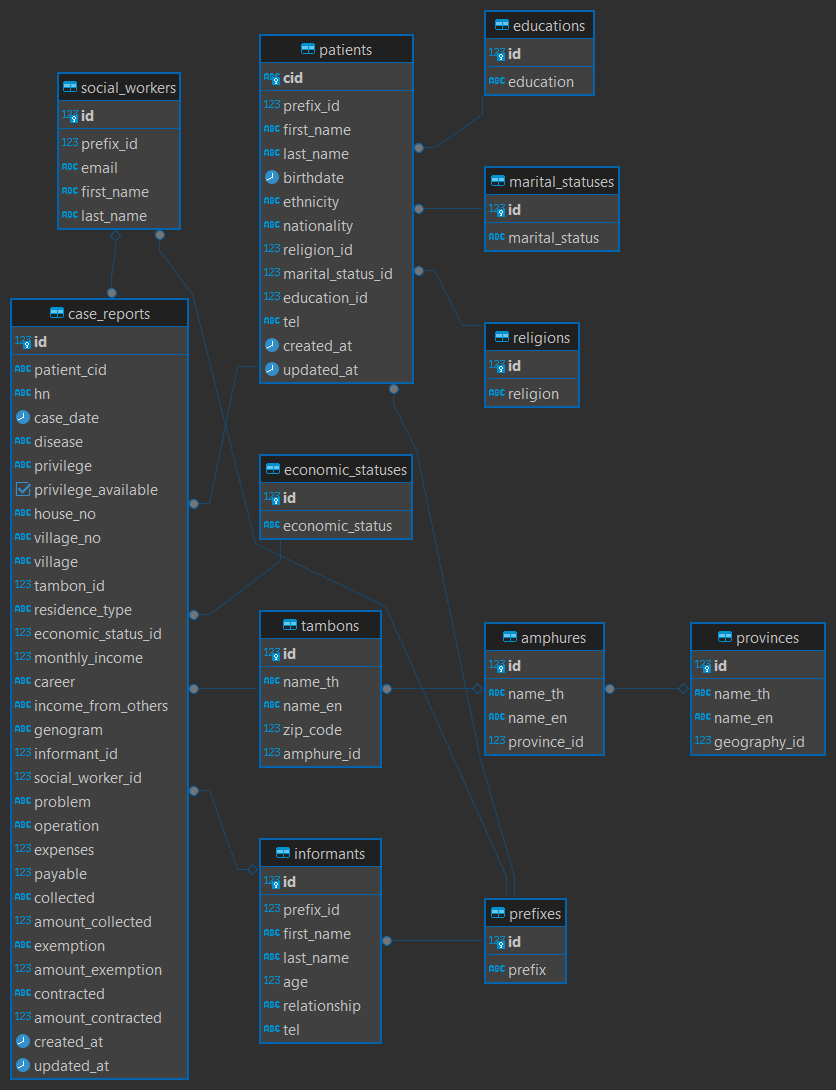
\includegraphics[width=1\textwidth]{481858458_4043514635914838_3135881775907933051_n.png}
  \end{center}
  \caption[โครงสร้างของฐานข้อมูล]{โครงสร้างของฐานข้อมูล}
\end{figure}
\newpage

\subsection{ข้อมูลผู้ป่วย}
โดยผู้ป่วย 1 คนจะมีข้อมูลได้แค่ 1 ข้อมูล
\subsection{ข้อมูลเคส}
โดยผู้ป่วย 1 คนสามารถมีได้หลายเคส (one to many)
\subsection{ข้อมูลนักสังคมสงเคราะห์}
โดยนักสังคมสงเคราะห์ 1 คนจะมีข้อมูลได้แค่ 1 ข้อมูล
\subsection{ข้อมูลผู้กรอก}
โดยเคส 1 เคสจะมีข้อมูลผู้กรอกได้แค่ 1 คนโดยอาจจะเป็นผู้ป่วยกรอกเองหรือญาติกรอกก็ได้
\subsection{ข้อมูลที่ใช้ทำ Drop-down Box}
ข้อมูลบางชนิดจะถูกเก็บไว้ในฐานข้อมูล แล้วจะถูกเรียกใช้ใน Drop-down Box เพื่อลดข้อผิดพลาดจากการพิมพ์ของนักสังคมสงเคราะห์
\begin{itemize}
\item educations
\item marital\_statuses
\item economic\_statuses
\item religions
\item prefixes
\item provinces
\item amphures
\item tambons
\end{itemize}